\begin{titlepage}

\begin{center}
{
\large \textbf{ Universit\'e Paul Sabatier, Toulouse  }

\vspace{0.5cm}

\begin{figure}[h] 
    \begin{center}
    
\includegraphics[width=0.1\textwidth]{Figures/Uni.png}
    \hspace{3cm}
    
\includegraphics[width=0.2\textwidth]{Figures/IMFT_Logo.pdf}
    \end{center}
\end{figure} 

\vspace{0.5cm}

\textbf{Institut de M\'ecanique des Fluides de Toulouse}

\vspace{1cm}

\Huge \textbf{\'Ecrire un rapport}

\vspace{0.5cm}
\Large
Obtenir une compétence transversale durant ces études supérieures.

}

\vspace{0.5cm}

\textbf{Christophe  Airiau }

\vspace{1cm}

Christophe.Airiau@imft.fr

\vspace{0.5cm}

\today


\begin{figure}[h] 
    \begin{center}
    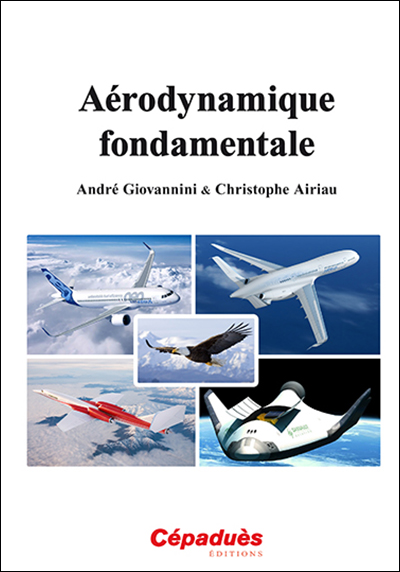
\includegraphics[width=0.2\textwidth]{Figures/Livre1.jpg}
    \hspace{3cm} 
    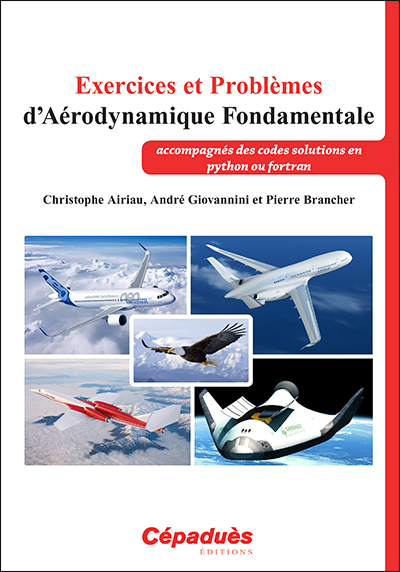
\includegraphics[width=0.2\textwidth]{Figures/Livre2.jpg}
    \end{center}
\end{figure} 

{\scriptsize 
\setstretch{0.4}
\begin{itemize}
\item \rouge{Ne pas hésiter à ajouter de jolies figures ou photos en page de titre, en lien avec le rapport}
\item \rouge{mettre les logos et le nom de l'organisme d'accueil}
\item \rouge{mettre une date avec éventuellement la mention provisoire, ou la version}
\item Titre expressif en gras, éventuellement ajouter un sous-titre, nom des auteurs et affiliation
\item \rouge{Ajouter le nom des encadrants avec affiliation}
\item Mise en forme: choix personnel ou imposé par le commanditaire ou organisme d'accueil
\end{itemize}
}
\end{center}
\end{titlepage}
